\documentclass[11pt]{article}
\usepackage{graphicx}
\usepackage{array}
\usepackage{xcolor}
\usepackage[a4paper,total={8in,10in}]{geometry}
\usepackage{mdframed}
\usepackage{geometry}
\usepackage{hyperref}
\begin{document}
\begin{mdframed}[backgroundcolor=orange]
~
\begin{center}
\begin{Huge}
\color{white}{\fontfamily{pbk}\selectfont SIDDHANT}\color{gray}{\fontfamily{pbk}\selectfont\textbf{ BHAMBRI}}
\end{Huge}
\end{center}
\begin{center}
\begin{large}
\color{white}\emph{Aiming to use technology to bring a considerable positive change for mankind}
\end{large}
\end{center}
\end{mdframed}
\begin{minipage}{1.00\linewidth}
\begin{center}
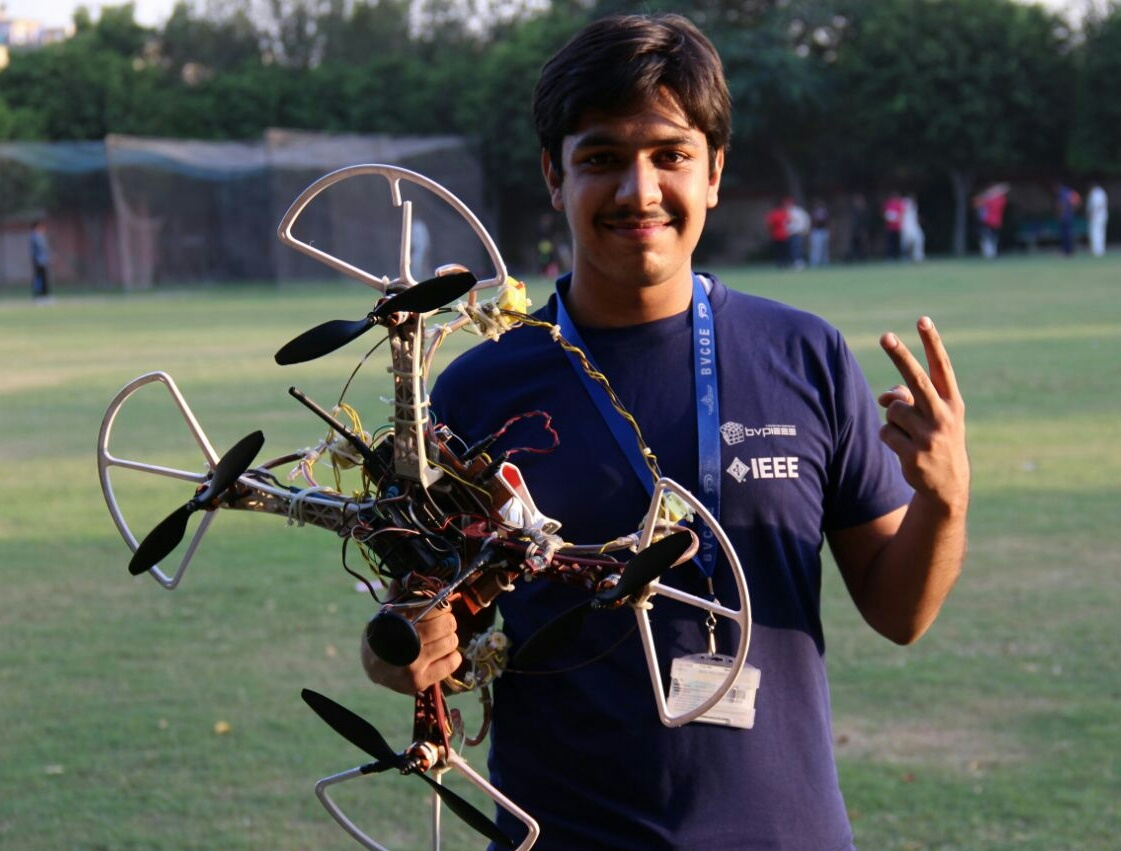
\includegraphics[scale=0.169]{siddhant_image}
\end{center}

\begin{flushleft}
\section{\color{red}Car\color{purple}e\color{black}er Obje\color{purple}ct\color{black}ive}
~
To secure the rewarding internship at e-Yantra, where I can be mentored by the experts in the field of the\\ ~ embeded system at IIT-Bombay which will be salutary for me to secure a career as a researcher in this field.
	\section{\color{green}Per\color{purple}s\color{black}onal D\color{purple}e\color{black}tai\color{purple}l\color{black}s}
	~
\textbf{Address-}    
    886/2A 
    Preet Vihar, Rohtak.\\
    ~
    Haryana\\
    ~
    124001\\
    ~
    \textbf{Contact}-
    +91 9728466229\\
~
\textbf{E-mail-} \href{mailto:siddhantbhambri@gmail.com}{siddhantbhambri@gmail.com}\\
 ~   
    \textbf{LinkedIn-}
    \href{http://www.linkedin.com/in/siddhant-bhambri-27b7a5111}{http://www.linkedin.com/in/siddhant-bhambri-27b7a5111}
\end{flushleft}

\section{\color{yellow}Edu\color{black}cational Qualifications}
\begin{center}
\begin{tabular}{ |m{4cm}| m{4cm}| m{2cm}| m{3cm}| }
\hline
&&&\\
\begin{center}
\textbf{{ Course/Examination }}
\end{center}&\begin{center}\textbf{ Institute/University }\end{center}&\begin{center}\textbf{ Year of passing }\end{center}&\begin{center}\textbf{ Performance }\end{center}\\
\hline
&&&\\
\begin{center}
B.Tech, Electronics and Communication Engineering
\end{center}& \begin{center}
Bharati Vidyapeeth's College Of Engineering
\end{center}&\begin{center}
2019
\end{center}& \begin{center}
71.00 (C) (up to third semester)
\end{center}\\
\hline
\begin{center}
CBSC (SCIENCE-PCM)\\
XIIth
\end{center}&
\begin{center}
(CBSE) Model School Rohtak, Haryana
\end{center}&
\begin{center}
2015
\end{center}&
\begin{center}
77.00 percent(agg)
\end{center}\\
\hline
\begin{center}
CBSE\\
Xth
\end{center}&
\begin{center}
(CBSE) Model School Rohtak, Haryana
\end{center}&
\begin{center}
2013
\end{center}&
\begin{center}
8.8 CGPA
\end{center}\\
\hline
\end{tabular}
\end{center}
\end{minipage}

\begin{minipage}{1.0\linewidth}

\section{\color{orange}Pro\color{black}jects}
\subsection{Co\color{purple}m\color{black}pl\color{purple}e\color{black}ted}
\begin{enumerate}
\item Model a Terrain using Serial communication between Firebird V and\\ Blender Game Engin using (XBees 2.4C).
\item Autonomous features like auto landing and take-off, Geo-fencing and\\ altitude hold in a multi-copter.
Link for Project - https://www.youtube.com/watch?v=N8zVc11KKoU
\item Quadcopter system for aerial surveillance using KK2.1.5 board. \\Link for Project - https://www.youtube.com/watch?v=N8zVc11KKoU
\item Bluetooth Controlled Quadcopter Rover Mechanisum using Arduino.
\item IOT based Plug AND Play Home Automation System Without Rewiring.
\item Wearable sensor module for gesture recognition and gait tracking. 
\item Making and controlling 8*8*8 multiplexed LED cube matrix with self-built PCB.
\item Tic-tac-toe Game with GUI(Graphic User Interface) in JAVA.
\item RFID, IR sensor,GSM and GPS based anti-car theft system.
\item Propeller Clock  (ATMEGA-8).
\item IoT based Door lock system (TI- CC3200).
\end{enumerate}
\subsection{Currently Working On}
\begin{enumerate}
\item Semi-Automated Car and self driving car system using (Raspberry Pi and\\ DIP). 
\item IOT based Plug AND Play Home Automation System Without Rewiring. 
\item HEX-Copter.
\item LifeLine (A medical alert app). 
\item Visible Light Communication(VLC)- Advanced version of LiFi
\end{enumerate}

\section{\color{magenta}Tra\color{black}ining and Internships}
\begin{enumerate}
\item \textbf{Industrial Training on Embedded Systems} (Cyborg Labs) [June-August 2016]
\item {Workshop series by Technex'17, IIT Varanasi on Internet of Things}[September 2016]
\item 14 hr. workshop series by Texas Instruments Ltd. On Embedded Systems and\\ Internet of Things[October 2016]
\item \textbf{Workshops on Arduino based controlling}/Robotic workshops(8) by RAS,\\ BVPIEEE [October 2016-Present]
\item \textbf{Complete JAVA masterclass} (Udemy) [Present 2017]
\item \textbf{Machine Learning by Andrew Ng\\ Created by Stanford university} (Coursera) [Present 2017]
\item \textbf{Workshops on Angular Js} by Brain Mentors Pvt.Ltd.
\item \textbf{Workshops on FPGA} (Field-Programmable gate array) [January 2017-]

\end{enumerate}
\end{minipage}

\begin{minipage}{1.5\linewidth}

\section{\color{blue}Res\color{black}earch, Publications and Patent's}
\begin{enumerate}
\item \textbf{Provisional Patent on non-rewiring based home automation system \\(Status-Awaiting Evaluation)
/item Patent on }
\end{enumerate}

\section{\color{cyan}Tec\color{black}hnical Skills}
\subsection{Programming Languages}
\begin{itemize}
\item C++
\item JAVA
\item Python Basics
\item Embedded C
\end{itemize}

\subsection{Operating Systems}
\begin{itemize}
\item macOS Sierra, version 10.12.3
\item Windows XP/7/8/10
\item Android
\end{itemize}
\subsection{Software and Platforms worked upon}
\begin{itemize}
\item Arduino IDE
\item Proteus
\item JDK(Java Development Kit)
\item Intelli IDEA CE
\item PyCharm CE
\item Microsoft Office
\item Energia
\item TeraTerm
\item XCTU
\item KK multicopter flash tool
\item Fritzing
\item LaTeX
\end{itemize}
\subsection{Others}
\begin{itemize}
\item Orcad Capture
\item AVR Studio
\item Blender Game Engine
\end{itemize}
\end{minipage}

\begin{minipage}{1.5\linewidth}
\subsection{Development Boards/Modules}
\begin{itemize}
\item ATMEGA16
\item Arduino Mega(ATMega 2560) and Uno(ATMega328)
\item MSP430(LaunchPad)
\item CC3200(built in accelerometer)
\item HC05
\item MPU 6050
\item Xbee
\end{itemize}

\section{\color{orange}Sof\color{black}t skills}
\begin{enumerate}
\item Fluent in Hindi and English, Hindi being the native language.
\item Research and Development Head Robotics and Automation Society, teaching experience to \\50+ fellow students.
\end{enumerate}

\section{\color{red}Ext\color{black}ra Curricular Activities}
\begin{itemize}
\item Senior Diploma in vocal music.
\item State Level Finalist in Singing Sanoni Foundation.
\item Head (Research And Development) BVPIEEE.
\item Student Member (Computer Society of India).
\item Student Member IEEE(Institute of Electrical and Electronics Engineers).
\end{itemize}


\section{\color{green}Co-C\color{black}urricular Activities}
\begin{enumerate}
\item \textbf{Positioned First in Model a Terrain Theme: e-Yantra 2016} \\(national level robotics competition  by IIT-Bombay) 
\item \textbf{Research  and  Development Head} at BVPIEEE RAS (July 2016-Present)
\item \textbf{Event Coordinator} at Robo Soccer event by BVPIEEE RAS, BVEST 2016 \\(October 2016)
\item \textbf{Event Manager} at robotic event (Guardians of Galaxy) at Fervour'16 (April 2016)
\item \textbf{Second position} holder at RoboThon Bvest,(BVCOE, October 2015)
\item \textbf{Second position} holder at RoboMaze Bvest,(BVCOE, October 2015)
\item \textbf{Technical Head} at robotic event (Maze solver) in Fervour'16 (April 2016)

\end{enumerate}
\end{minipage}

\begin{minipage}{1.5\linewidth}
\section{\color{yellow}Per\color{black}sonal Details}
\begin{tabular}{l l}
\textbf{Father's Name}-& Mr. Viney Bhambri\\ 
\textbf{Mother's Name}-& Mrs. Ashita Bhambri\\
\textbf{Sex}-& Male\\
\textbf{Date of Birth}-& 13/04/1997\\
\textbf{Nationality}-& Indian\\
\textbf{Marital Status}-& Unmarried\\
\end{tabular}
\section{\color{magenta}Ref\color{black}rences}
\begin{itemize}
\item Mr. Abhishek Gagneja, Assistant Professor, Bharati Vidyapeeth's College of Engineering\\
Contact no.- +91 9971122557
\item Mr. Ashish Kumar, Assistant Professor, Bharati Vidyapeeth's College of Engineering\\
Contact no.- +91 9810955760
\item Mr. Shivam Bhardwaj, Ex-Vice Chairperson (BVPIEEE),\\Ex-Chairperson (BVPIEEE-RAS) and CTO (REES 52)
Contact No.: +91 8130844448
\item Mr. Dhruv Gaba, Ex-Vice Chairperson (BVPIEEE-RAS) and CRO (REES 52)\\
Contact No.: +91 8527553713

\end{itemize}

\section{\color{green}Dat\color{black}e}
24/04/2017

\end{minipage}

\end{document}